\section{Self-Practice A12}

\begin{problem}
    Two events $A$ and $B$ are such that $\P{A} = 0.6$, $\P{B} = 0.3$, $\P{A}{B} = 0.2$. Calculate the probabilities that
    \begin{enumerate}
        \item both events occur,
        \item at least one of the two events occurs,
        \item exactly one of the events occur.
    \end{enumerate}
\end{problem}
\begin{solution}
    \begin{ppart}
        $\P{A \cap B} = \P{B} \P{A}{B} = (0.2)(0.3) = 0.06$.
    \end{ppart}
    \begin{ppart}
        $\P{A \cup B} = \P{A} + \P{B} - \P{A \cap B} = 0.6 + 0.3 - 0.06 = 0.84$.
    \end{ppart}
    \begin{ppart}
        The required probability is given by $\P{A \cup B} - \P{A \cap B} = 0.84 - 0.06 = 0.78$.
    \end{ppart}
\end{solution}

\begin{problem}
    For events $A$ and $B$, it is given that $\P{A} = 0.7$, $\P{B}{A'} = 0.8$, $\P{A}{B'} = 0.88$. Find
    \begin{enumerate}
        \item $\P{B \cap A'}$,
        \item $\P{A' \cap B'}$,
        \item $\P{A \cap B}$.
    \end{enumerate}
\end{problem}
\begin{solution}
    \begin{ppart}
        $\P{B \cap A'} = \P{A'} \P{B}{A'} = \bp{1 - 0.7}(0.8) = 0.24$.
    \end{ppart}
    \begin{ppart}
        Note that $\P{B'}{A'} = 1 - \P{B}{A'}$. Hence, $\P{B' \cap A'} = \P{A'} \P{B'}{A'} = \bp{1 -0.7} \bp{1 - 0.8} = 0.06$.
    \end{ppart}
    \begin{ppart}
        Let $x = \P{A \cap B}$. Then $\P{A \cap B'} = \P{A} - x = 0.7 - x$, so \[0.88 = \P{A}{B'} = \frac{\P{A \cap B'}}{\P{B'}} = \frac{\P{A \cap B'}}{\P{A \cap B'} + \P{A' \cap B'}} = \frac{0.7 - x}{\bp{0.7 - x} + 0.06},\] which yields $x = \P{A \cap B} = 0.26$ upon simplification.
    \end{ppart}
\end{solution}

\begin{problem}
    A group of student representatives is to be chosen from three schools, $R$, $S$ and $T$. The group is to consist of 10 students and is chosen from a set of 15 students consisting of 3 from $R$, 4 from $S$ and 8 from $T$. Find the probability that the group consists of
    \begin{enumerate}
        \item students from $S$ and $T$ only,
        \item at least one student from each school.
    \end{enumerate}
\end{problem}
\begin{solution}
    \begin{ppart}
        There are $\comb{15}{10}$ ways to form a group without restriction, and there are $\comb{4+8}{10}$ ways to form a group consisting of students from only $S$ and $T$. Thus, the desired probability is $\comb{4+8}{10}/\comb{15}{10} = 2/91$.
    \end{ppart}
    \begin{ppart}
        Consider the complement, i.e. the event that at least one school has no representative. The only way this can happen is if the group consists of students from $R$ and $T$ only, or from $S$ and $T$ only. Thus, the required probability is \[1 - \frac{\comb{3 + 8}{10} + \comb{4 + 8}{10}}{\comb{15}{10}} = \frac{38}{39}.\]
    \end{ppart}
\end{solution}

\begin{problem}
    A box contains 25 apples, of which 20 are red and 5 are green. Of the red apples, 3 contain maggots and of the green apples, 1 contains maggots. Two apples are chosen at random from the box. Find, in any order,
    \begin{enumerate}
        \item the probability that both apples contain maggots.
        \item the probability that both apples are red and at least one contains maggots.
        \item the probability that at least one apple contains maggots, given that both apples are red.
        \item the probability that both apples are red given that at least one apple is red.
    \end{enumerate}
\end{problem}
\begin{solution}
    \begin{ppart}
        The required probability is \[\frac{4}{25} \times \frac{3}{24} = \frac{1}{50}.\]
    \end{ppart}
    \begin{ppart}
        The required probability is \[\P{\text{both red}} - \P{\text{both red and no maggot}} = \frac{20}{25} \times \frac{19}{24} - \frac{17}{25} \times \frac{16}{24} = \frac9{50}.\]
    \end{ppart}
    \begin{ppart}
        The required probability is \[\frac{\P{\text{both red and at least one maggot}}}{\P{\text{both red}}} = \frac{9/50}{(20/25) \times (19/24)} = \frac{27}{95}.\]
    \end{ppart}
    \begin{ppart}
        The required probability is \[\frac{\P{\text{both red}}}{\P{\text{at least one red}}} = \frac{\P{\text{both red}}}{1 - \P{\text{both green}}} = \frac{(20/25) \times (19/24)}{1 - (5/25)(4/24)} = \frac{19}{29}.\]
    \end{ppart}
\end{solution}

\begin{problem}
    A bag contains 15 tokens that are indistinguishable apart from their colours. 2 of the tokens are blue and the rest are either red or green. Participants are required to draw the tokens randomly, one at a time, from the bag without replacement.

    \begin{enumerate}
        \item Given that the probability that a participant draws 2 red tokens on the first 2 draws is $1/35$, show that there are 3 red tokens in the bag.
        \item Find the probability that a participant draws a red or green token on the second draw.
    \end{enumerate}

    Events $A$ and $B$ are defined as follows.
    \begin{itemize}
        \item $A$: A participant draws his/her second red token on the third draw.
        \item $B$: A participant draws a blue token on the second draw.
    \end{itemize}

    \begin{enumerate}
        \setcounter{enumi}{2}
        \item Find $\P{A \cup B}$.
        \item Determine if $A$ and $B$ are independent events.
    \end{enumerate}
\end{problem}
\begin{solution}
    \begin{ppart}
        Let $r$ be the number of red tokens. Then \[\P{\text{2 red tokens on second draw}} = \frac{r}{15} \times \frac{r-1}{14} = \frac1{35}.\] This gives $r^2 - r - 6 = (r-3)(r+2) = 0$, so $r = 3$. Note that we reject $r = -2$ since $r \geq 0$.
    \end{ppart}
    \begin{ppart}
        We have \[\P{\text{red/green on 2nd draw}} = \frac{13}{15} \times \frac{12}{14} + \frac{2}{15} \times \frac{13}{14} = \frac{13}{15}.\]
    \end{ppart}
    \begin{ppart}
        We have \[\P{A} = \frac{3}{15} \times \frac{12}{14} \times \frac{2}{13} + \frac{12}{15} \times \frac{3}{14} \times \frac{2}{13} = \frac{24}{455}\] and \[\P{B} = 1 - \P{\text{red/green on 2nd draw}} = 1 - \frac{13}{15} = \frac{2}{15}.\] Note that the event $A \cap B$ can only occur if the first and third draws are red, and the second draw is blue. Thus, \[\P{A \cap B} = \frac{3}{15} \times \frac{2}{14} \times \frac{2}{13} = \frac{2}{455}.\] Thus, \[\P{A \cup B} = \P{A} + \P{B} - \P{A \cap B} = \frac{24}{455} + \frac{2}{15} - \frac{2}{455} = \frac{248}{1365}.\]
    \end{ppart}
    \begin{ppart}
        Observe that \[\P{A} \P{B} = \frac{24}{455} \times \frac{2}{15} = \frac{16}{2275} \neq \frac{248}{1365} = \P{A \cap B}.\] Thus, $A$ and $B$ are not independent.
    \end{ppart}
\end{solution}

\clearpage
\begin{problem}
    \begin{center}\tikzsetnextfilename{352}
        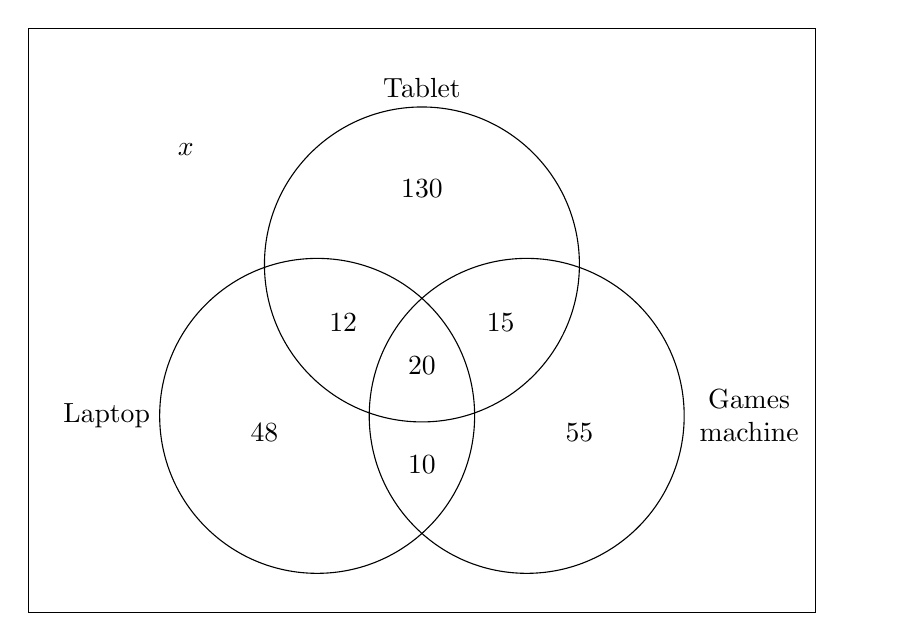
\begin{tikzpicture}
            \coordinate (A) at (-5, -0.5/1.3 - 2.5);
            \coordinate (B) at (5, -0.5/1.3 - 2.5);
            \coordinate (C) at (5, 2/1.3 + 3);
            \coordinate (D) at (-5, 2/1.3 + 3);

            \draw (A) -- (B);
            \draw (B) -- (C);
            \draw (C) -- (D);
            \draw (D) -- (A);

            \draw (0,2/1.3) circle[radius=2];
            \draw (-1.73/1.3,-0.5/1.3) circle[radius=2];
            \draw (1.73/1.3,-0.5/1.3) circle[radius=2];

            \node[left] at (-1.73/1.3 - 2,-0.5/1.3) {Laptop};
            \node[right, text width=3cm,align=center] at (1.73/1.3 + 1.2,-0.5/1.3) {Games\\machine};
            \node[above] at (0,2/1.3+2) {Tablet};

            \node at (-3, 3) {$x$};
            \node at (0, 2.5) {130};
            \node at (-2, -0.6) {48};
            \node at (2, -0.6) {55};
            \node at (-1, 0.8) {12};
            \node at (0, -1) {10};
            \node at (1, 0.8) {15};
            \node at (0, 0.25) {20};
        \end{tikzpicture}
    \end{center}

    A group of students is asked whether they own any of a laptop, a tablet and a games machine. The numbers owning different combinations are shown in the Venn diagram. The number of students owning none of these is $x$. One of the students is chosen at random.
    
    \begin{itemize}
        \item $L$ is the event that the student owns a laptop.
        \item $T$ is the event that the student owns a tablet.
        \item $G$ is the event that the student owns a game machine.
    \end{itemize}

    \begin{enumerate}
        \item Write down expressions for $\P{L}$ and $\P{G}$ in terms of $x$. Given that $L$ and $G$ are independent, show that $x = 10$.
    \end{enumerate}

    Using this value of $x$, find
    \begin{enumerate}
        \setcounter{enumi}{1}
        \item $\P{L \cup T}$,
        \item $\P{T \cap G'}$,
        \item $\P{L}{G}$.
    \end{enumerate}

    Two students from the whole group are chosen at random.
    
    \begin{enumerate}
        \setcounter{enumi}{4}
        \item Find the probability that both of these students each owns exactly two out of the three items (laptop, tablet, games machine).
    \end{enumerate}
\end{problem}
\begin{solution}
    \begin{ppart}
        We have \[\P{L} = \frac{90}{290 + x}, \quad \P{G} = \frac{100}{290 + x}, \quad \P{L \cap G} = \frac{30}{290 + x}.\] Since $L$ and $G$ are independent, $\P{L}\P{G} = \P{L \cap G}$, so \[\frac{90}{290 + x} \times \frac{100}{290 + x} = \frac{30}{290 + x}.\] Solving, we get $x = 10$.
    \end{ppart}
    \begin{ppart}
        We have \[\P{L \cup T} = \frac{235}{300} = \frac{47}{60}.\]
    \end{ppart}
    \begin{ppart}
        We have \[\P{T \cap G'} = \frac{143}{300} = \frac{71}{150}.\]
    \end{ppart}
    \begin{ppart}
        We have \[\P{L}{G} = \frac{\P{L \cap G}}{\P{G}} = \frac{30/300}{100/300} = \frac{3}{10}.\]
    \end{ppart}
    \begin{ppart}
        Observe that the number of students that own exactly two items is $12 + 15 + 10 = 37$. The required probability is hence \[\frac{37}{300} \times \frac{36}{299} = \frac{111}{7475}.\]
    \end{ppart}
\end{solution}

\begin{problem}
    A group of students takes an examination in Science. A student who fails the examination at the first attempt is allowed one further attempt. For a randomly chosen student, the probability of passing the examination at the first attempt is $p$. If the student fails the examination at the first attempt, the probability of passing at the second attempt is $0.3$ more than the probability of passing the examination at the first attempt.

    \begin{enumerate}
        \item Show that the probability that a randomly chosen student passes the examination is $0.3 + 1.7p - p^2$.
    \end{enumerate}

    Find the value of $p$ such that the probability that a randomly chosen student passes the examination on the first attempt given that the student passes is $0.6$.

    Two students are randomly chosen.

    \begin{enumerate}
        \setcounter{enumi}{1}
        \item \begin{enumerate}
            \item Find the probability that one passes the examination on the first attempt and the other passes the examination on the second attempt, leaving your answer in terms of $p$.
            \item Find the value of $p$ such that the value of the probability in part (i) is maximum.
        \end{enumerate}
    \end{enumerate}
\end{problem}
\begin{solution}
    \begin{ppart}
        We have $\P{\text{pass}} = p + \bp{1 - p}\bp{p + 0.3} = -p^2 + 1.7p + 0.3$.
    \end{ppart}
    \begin{ppart}
        We have \[\P{\text{pass on 1st attempt}}{\text{pass}} = \frac{\P{\text{pass on 1st attempt}}}{\P{\text{pass}}} = \frac{p}{-p^2 + 1.7p + 0.3}.\] Equating this to $0.6$, we get $p = 0.565$ or $p = -0.531$, which we reject since $p \in [0, 1]$. Thus, the desired probability is $p = 0.565$.
    \end{ppart}
    \begin{ppart}
        The required probability is $2\bs{p \times \bp{1-p}\bp{p+0.3}} = -2p^3 + 1.4p^2 + 0.6p$.
    \end{ppart}
    \begin{ppart}
        Let $f(p) = -2p^3 + 1.4p^2 + 0.6p$. For stationary points, \[\der{f}{p} = -6p^2 + 2.8p + 0.6 = 0,\] which occurs when $p = 0.626$. Note that we reject $p = -0.160$ since $p \in [0, 1]$. At $p = 0.626$, the second derivative is \[\evalder{\der[2]{f}{p}}{p=0.626} = \evalder{\bp{-12p + 2.8}}{p = 0.626} = -4.712 < 0,\] thus the probability is maximum at $p = 0.626$.
    \end{ppart}
\end{solution}

\begin{problem}
    In Haha College, 70\% of the students watch the show \textit{Jogging Man} and 60\% of the students watch the show \textit{Voice of Me}. 40\% of those who do not watch the show \textit{Voice of Me} watch the show \textit{Jogging Man}. Find the probability that a student chosen at random from the college
    \begin{enumerate}
        \item watches both shows,
        \item watches exactly one show,
        \item watches the show \textit{Voice of Me} given that the student does not watch the show \textit{Jogging Man}.
    \end{enumerate}

    State, with a reason, whether the events `watches \textit{Jogging Man}' and `watches \textit{Voice of Me}' are independent.
\end{problem}
\begin{solution}
    Let $J$ be the event that a student watches \textit{Jogging Man}, and $V$ be the event that a student watches \textit{Voice of Me}. We have $\P{J} = 0.7$, $\P{V} = 0.6$ and $\P{J}{V'} = 0.4$.

    \begin{ppart}
        We have $\P{J \cap V'} = \P{V'} \bp{J}{V'} = \bp{1 - 0.6} \bp{0.4} = 0.16$. Thus, the probability that the student watches both shows is $\P{J \cap V} = \P{J} - \P{J \cap V'} = 0.7 - 0.16 = 0.54$.
    \end{ppart}
    \begin{ppart}
        The probability that the student watches exactly one show is
        \begin{align*}
            \P{J \cup V} - \P{J \cap V} &= \bp{\P{J} + \P{V} - \P{J \cap V}} - \P{J \cap V}\\
            &= \bp{0.7 + 0.6 - 0.54} - 0.54\\
            &= 0.22.
        \end{align*}
    \end{ppart}
    \begin{ppart}
        The desired probability is \[\P{V}{J'} = \frac{\P{V \cap J'}}{\P{J'}} = \frac{\P{V} - \P{V \cap J}}{1 - \P{J}} = \frac{0.6 - 0.54}{1 - 0.7} = 0.2.\]
    \end{ppart}

    Note that $\P{J \cap V} = 0.54 \neq (0.7)(0.6) = \P{J} \P{V}$, thus $J$ and $V$ are not independent.
\end{solution}

\begin{problem}
    For events $A$ and $B$, it is given that $\P{A} = 2/3$ and $\P{B} = 1/2$.
    
    \begin{enumerate}
        \item State an inequality satisfied by $\P{A \cap B}$.
    \end{enumerate}

    It is given further that $A$ and $B$ are independent. Find
    \begin{enumerate}
        \setcounter{enumi}{1}
        \item $\P{A \cap B}$,
        \item $\P{A' \cup B}$.
    \end{enumerate}
\end{problem}
\begin{solution}
    \begin{ppart}
        Note that \[\P{A \cap B} \leq \min{\P{A}, \P{B}} = \frac12.\] Further, \[\P{A \cup B} = \P{A} + \P{B} - \P{A \cap B} = \frac76 - \P{A \cap B},\] so $\P{A \cap B} \geq 1/6$. Putting both inequalities together, we have \[\frac16 \leq \P{A \cap B} \leq \frac12.\]
    \end{ppart}
    \begin{ppart}
        Since $A$ and $B$ are independent, \[\P{A \cap B} = \P{A} \P{B} = \frac23 \times \frac12 = \frac13.\]
    \end{ppart}
    \begin{ppart}
        We have \[\P{A' \cup B} = 1 - \P{A \cap B'} = 1 - \bp{\P{A} - \P{A \cap B}} = 1 - \bp{\frac23 - \frac13} = \frac23.\]
    \end{ppart}
\end{solution}

\begin{problem}[\chili]
    A fast food restaurant gives away a free action figure for every child's meal bought. There are five different action figures and each figure is equally likely to be given away with a child's meal. A customer intends to collect all five different figures by buying child's meals.

    \begin{enumerate}
        \item Find the probability that the first 4 child's meals bought by the customer all had different action figures.
        \item Two of the five action figures are X and Y. Find the probability that the first 4 action figures obtained result in the customer having at least one X or one Y or both.
        \item Find the probability that the first 4 child's meals bought by the customer had exactly two different action figures.
        \item At a certain stage, the customer collected 4 of the five action figures. Given that the probability of the customer completing the set by at most $n$ meals is larger than 0.95, find the least value of $n$.
    \end{enumerate}
\end{problem}
\begin{solution}
    \begin{ppart}
        Without restriction, there are $5^4$ ways to get action figures from four orders. If all four action figures are distinct, there are only $\perm{5}{4}$ ways to do so. The required probability is thus $\perm{5}{4} / 5^4 = 24/125$.
    \end{ppart}
    \begin{ppart}
        Consider the complement, i.e. the event that the first 4 action figures do not contain any X or Y. Since there are now only three possible action figures available, there are $3^4$ ways for this to happen. The required probability is then \[1 - \frac{3^4}{5^4} = \frac{544}{625}.\]
    \end{ppart}
    \begin{ppart}
        Let X and Y be the pair of action figures that the customer obtained. There are $\comb{5}{2}$ possible pairs. Since there are only two possible action figures available, there are $2^4$ ways to obtain at most two different action figures. Since there are 2 ways to get only one action figure (either all four orders are X's or Y's), the desired probability is \[\frac{\comb{5}{2} \bp{2^4 - 2}}{5^4} = \frac{28}{125}.\]
    \end{ppart}
    \begin{ppart}
        Consider the complement, i.e. the event that the customer does not complete his set by at most $n$ meals. This probability is given by $(4/5)^n$, so the desired inequality is \[1 - \bp{\frac45}^n \geq 0.95.\] Using G.C., the least $n$ is 14.
    \end{ppart}
\end{solution}